\chapter{Identyfikacja}
\label{cha:Identyfikacja}
%---------------------------------------------------------------------------

\section{Model matematyczny}
\label{sec:model_mat}
W celu wyznaczenia modelu matematycznego omawianego obiektu posłużono się rówaniami elektrycznym \ref{eq:elekt} oraz mechanicznym \ref{eq:mechaniczne} silnika
\begin{figure}[H]

	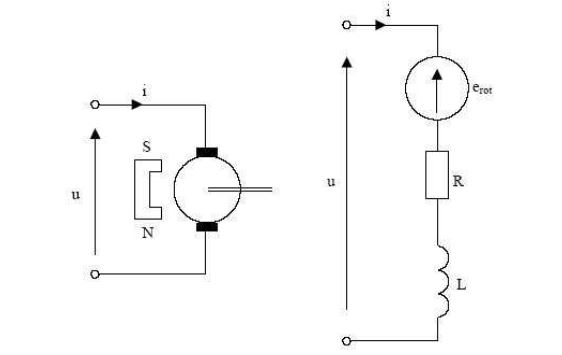
\includegraphics[width=0.5\textwidth]{identyfikacja/model_silnika}
	\centering
	\caption{Model silnika prądu stałego.}
	\label{fig:Schemat}
\end{figure}



\begin{equation}
\label{eq:elekt}
u(t)= R \cdot i(t) + L \frac{d}{dt}i(t) + e_{rot}
\end{equation}

\begin{equation}
\label{eq:mechaniczne}
J \cdot \frac{d}{dt} \omega(t) = K_{E} \cdot \phi \cdot i(t)
\end{equation}
gdzie:
\newline $e_{rot} = k_{E} \cdot \phi \cdot \omega(t)$

gdzie:

R - rezystancja uzwojeń twornika,
L - indukcyjność uzwojeń twornika,
$e_{rot}$ - siła elektromotoryczna,
J - moment bezwłądności silnika,
$\phi$ -strumień wzbuczenia od magnesów trwałych
$k_E$ - wsppółczynnik proporcjonalności wiążący napięcie rotacji z prędkością kątową oraz moment elektromagnetyczny z prądem twornika% TODO co to jest ?
 
%\begin{equation}
%\label{eq:e_rot}
%e_{rot} = k_{E} \cdot \phi \cdot \omega(t)
%\end{equation}

Skąd otrzymano układ równań silnika w postaci operatorowej postaci \ref{eq:oper}

\begin{equation}
\label{eq:oper}
\left\{ \begin{array}{ll}
U(s)  = R \cdot I(s) + L \cdot I(s) \cdot s + k_{E} \cdot \phi \cdot \Omega(s)\\
J \cdot \Omega(s) \cdot s  = K_{E} \cdot \phi \cdot I(s)
\end{array} \right.
\end{equation}

 Skąd po przekształceniach otrzymano wzór na transmitancję układu \ref{eq:transmitancja_pred}
\begin{equation}
\label{eq:transmitancja_pred}
G(s) = \frac{\Omega(s)}{U(s)} = \frac{K}{T \cdot s + 1}
\end{equation}

Jest to transmitancja obiektu pierwszego rzędu opisującą zależność obrotów silnika od napięcia wejściowgo, natomiast transmitancja \ref{eq:transmitancja_kat}:
\begin{equation}
\label{eq:transmitancja_kat}
G(s) = \frac{\alpha(s)}{U(s)} = \frac{ K}{s \cdot (T \cdot s + 1)}
\end{equation}
opisuje zależność kąta wału silnika od napięcia wejściowego. Jest to transmitancja obiektu inercyjnego z członem całkującym

\section{Martwa strefa}
W trakcie badań nad systemem zauważono, że występuje w nim zjawisko martwej strefy. Zostało ono przedstawione na rysunku \ref{fig:martwa_sterfa}
\begin{figure}[H]
	
	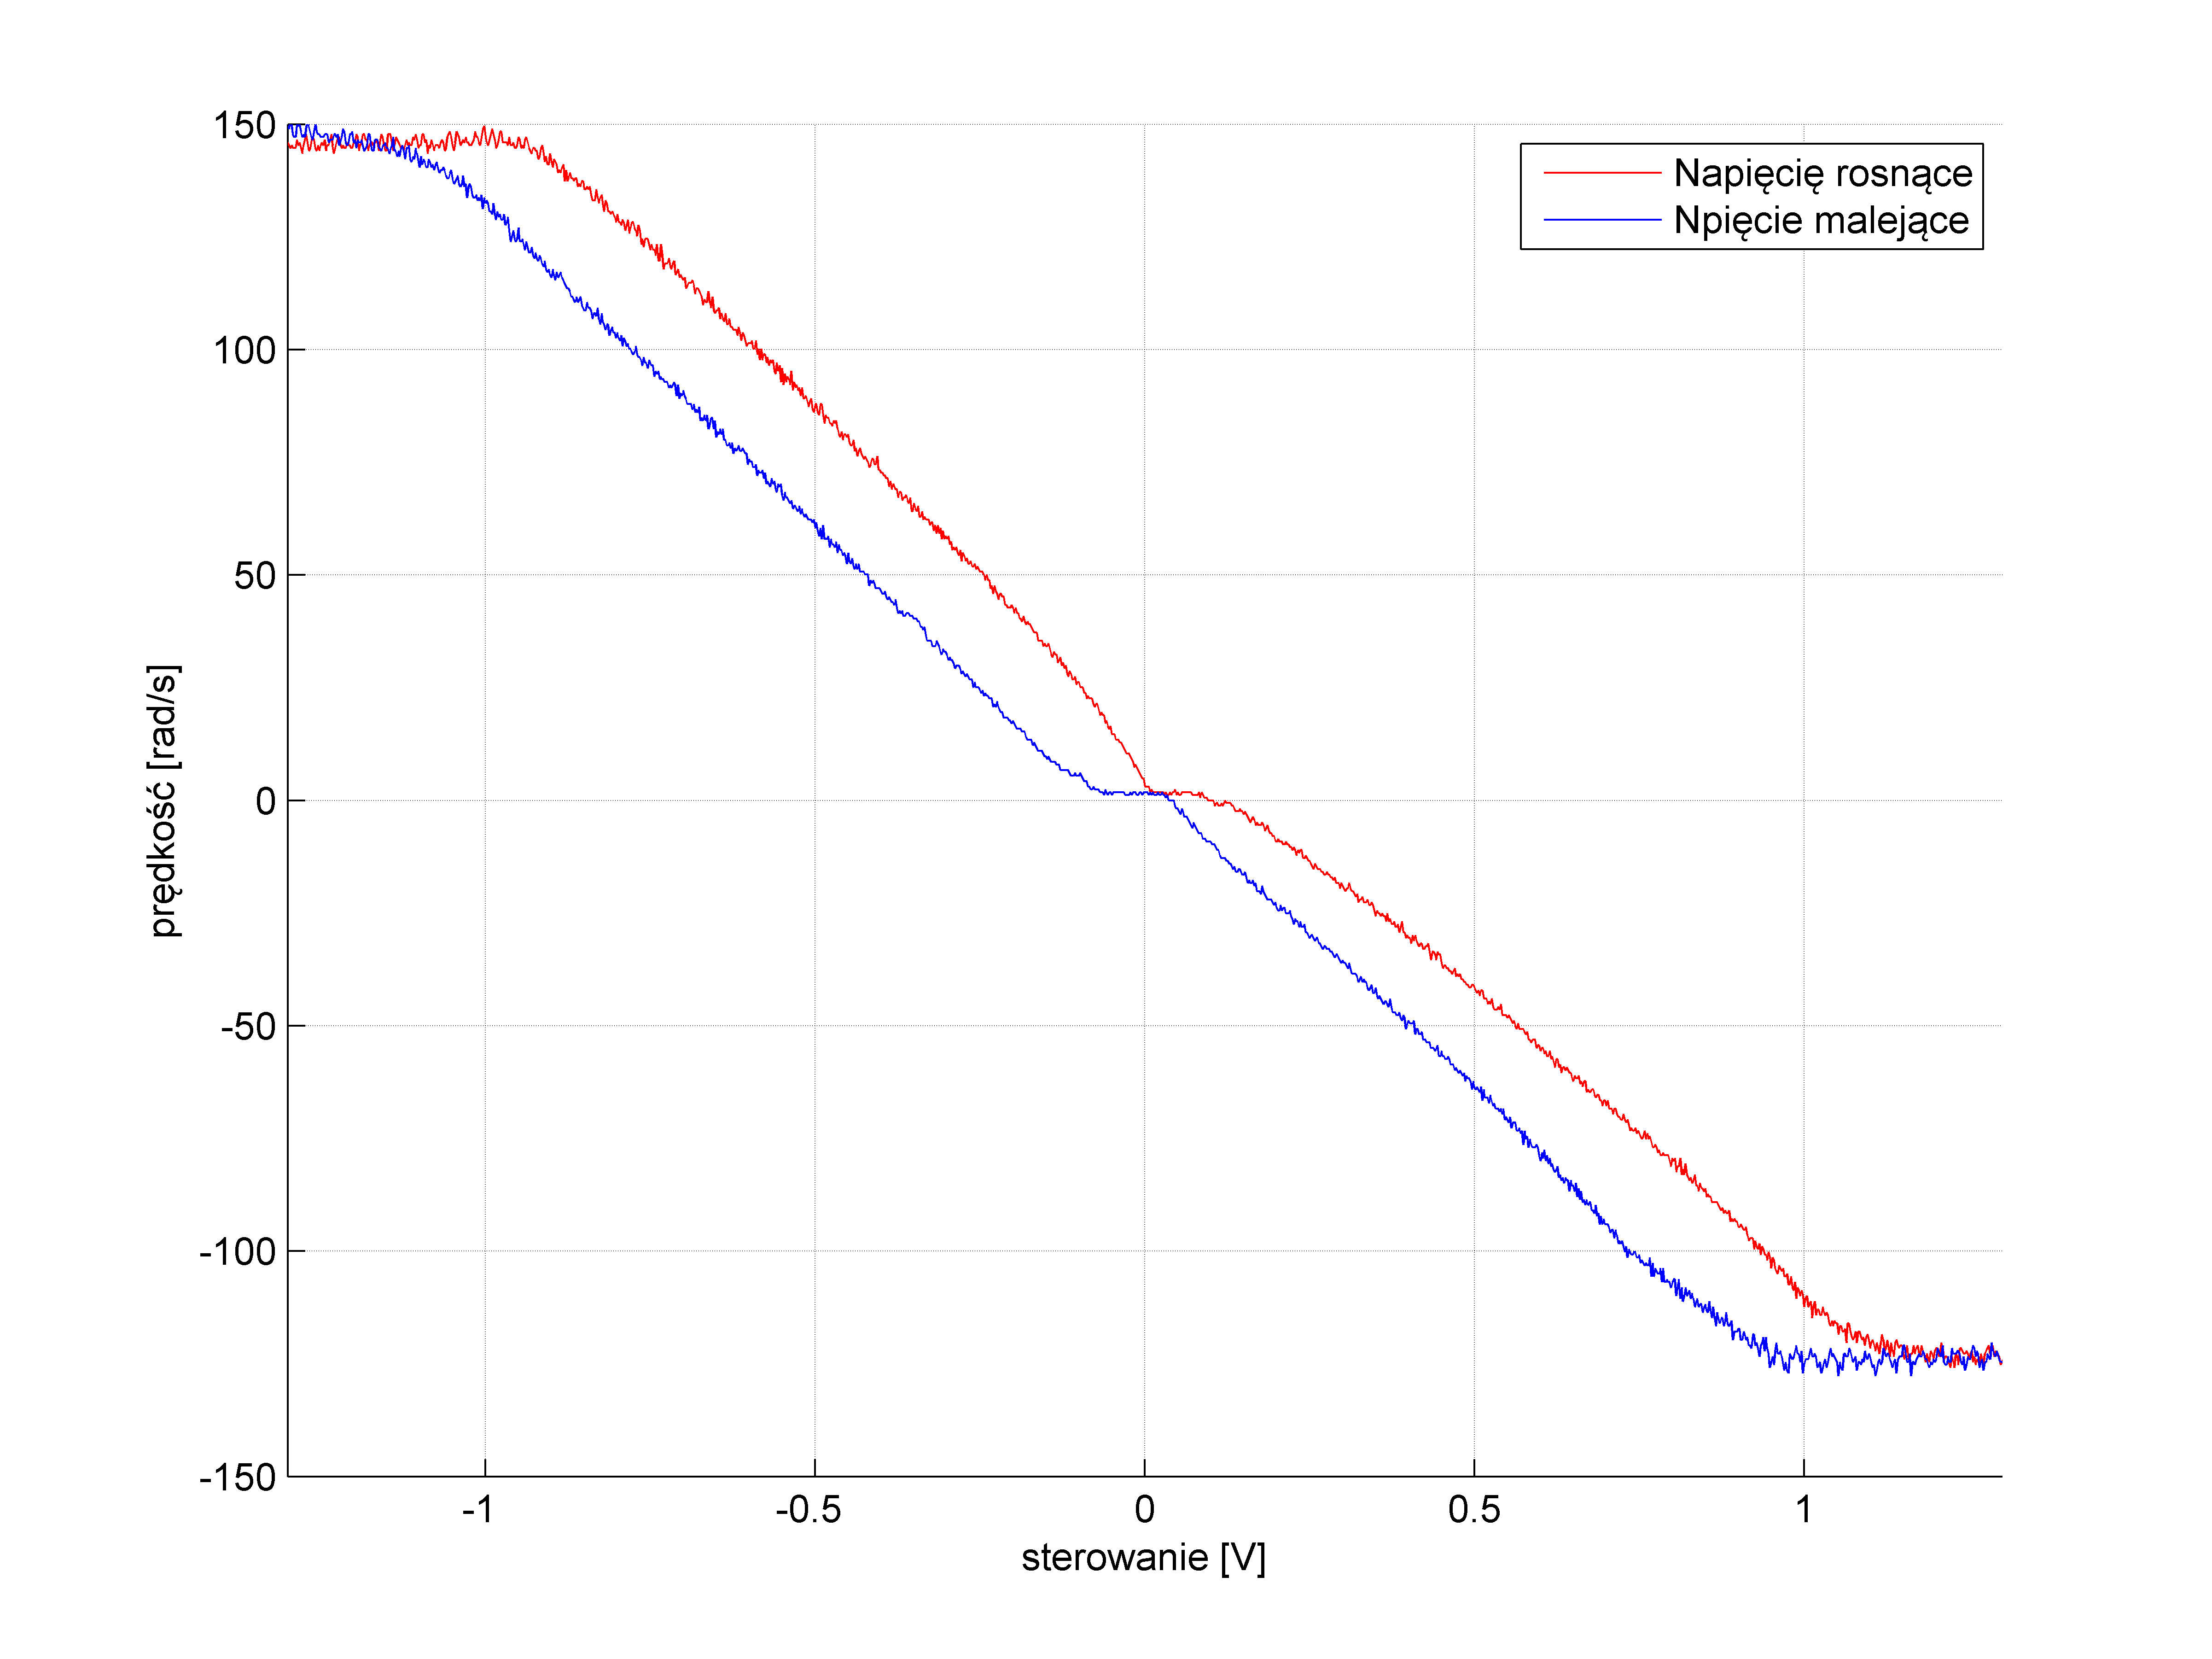
\includegraphics[width=0.7\textwidth]{identyfikacja/martwa_strefa}
	\centering
	\caption{Martwa strefa silnika.}
	\label{fig:martwa_sterfa}
\end{figure}

Na podstawie powyższego rysunku można stwierdzić iż silnik posiada niesymetryczną martwą strefę. Dla napięcia rosnącego źle źle źle źle!!!! w modelu nie uwzględniamy napięcia rosnącego lub malejącego tylko ujemne i dodatnie!!!! kurwa
\section{Modele}
\subsection*{Model z pojedynczej transmitancji}
\subsection*{Model z podwójnej transmitancji}
